\chapter{Realisierung}
% Dies ist das Hauptkapitel Ihrer Arbeit! Hier wird die Umsetzung der eigenen Ideen und Konzepte
% (Kapitel 3) anhand der gewählten Methoden (Kapitel 4) beschrieben, inkl. der dabei aufgetretenen
% Schwierigkeiten und Einschränkungen.
Die Realisierung lässt sich in drei Phasen unterteilen.

In der ersten Phase werden grundlegende Entscheidungen getroffen und die Basis der Arbeit implementiert.
Am Ende der ersten Phase existiert ein Prototyp,
welcher bei allen Komponenten des System die über minimale Funktionen verfügt. (TODO verweis )

Wie im Kapitel Vorgehen beschrieben (TODO), folgen darauf zwei weitere Phasen,
in welche neue Anforderungen des Auftraggebers umgesetzt werden.

\section{Grundlegende Designentscheidungen}

Der folgende Abschnitt gibt einen Überblick der gewählten Technologien und
der grundlegenden Designentscheidungen und wieso diese so umgesetzt wurden.

\subsection{Auswahl des Technologiestacks}

Bei er Auswahl des Technologiestacks wurde auf verschiedene Aspekte geachtet.
Zum einen sollte das Frontend unabhängig vom Backend entwickelt werden können.
Aus diesem Grund wurde für die Kommunikation, wie in Kapitel \ref{konzepte:api-kommunikation}
bereits beschrieben, eine \ac{REST} \ac{API} verwendet.
Auf die genaue Definition der \ac{API} wird in den nächsten Abschnitten noch genauer eingegangen.

Für die Implementation des Backends gibt es unzählige Technologien die man für eine \ac{CRUD}
Applikation verwenden kann (Siehe Kapitel \ref{state:backend}). Für dieses Projekt sollte
eine \ac{REST} \ac{API} implementiert werden können. Und die Datenbank soll über ein \ac{ORM}
abstrahiert werden können. Dies hat den Vorteil, dass die eigentliche Datenbanktechnologie
keine grosse Rolle spielt. Das \ac{ORM} abstrahiert die Tabellenstruktur mittels
Objekten im Sourcecode. Als Backend kann beispielsweise zum Testen und Entwickeln
eine Sqlite\footnote{https://www.sqlite.org/index.html} Datenbank verwendet werden.
Der gleiche Sourcecode kann danach in der Produktion auf eine PostgreSQL\footnote{https://www.postgresql.org/}
Datenbank zugreifen um besser zu skallieren.
Natürlich soll auch ein \ac{MQTT} Framework in der gewählten Technologie zur verfügung stehen
damit die Messdaten der Stromzähler empfangen und in die Datenbank abgespeichert werden können.

Python bietet für jedes dieser Anforderungen gleich mehrere Frameworks an. Mit Python können sehr
schnell Prototypen erstellt werden. Es eignet sich aber auch für grosse Produktivsoftware.
Einige der wohl Bekanntesten Programme wie YouTube, Instagram, Spotify oder Reddit sind
in Python geschrieben. \cite{popular_python_sw}

Bei der Implementation des Frontends wurde wie in Kapitel \ref{state:frontend} beschrieben
anhand der State of Js Umfragen React\footnote{https://reactjs.org/} verwendet.
Um nicht das ganze Benutzerinterface selber gestalten zu müssen, wurde eine Material Design\footnote{https://material.io/design}
Library verwendet.

Um die Applikation für die Entwicklung lokal aufzusetzen, zu testen oder zu Deployen wurde dazu
Podman verwendet (Siehe Kapitel \ref{state:deployment}).

\subsection{Datenbankschema}

Gleich zu beginn des Projektes wurde das Datenbankschema erstellt.
Dies gibt eine gute Übersicht ob die für das Projekt benötigten Daten
abgespeicher werden können. In diesem Fall sind das die Messwerte der Stromzähler
und die Labels des Benutzers.

Die Datenbank wurde so einfach wie möglich gehalten um alle vorgegebenen
Anforderungen zu erfüllen.

\begin{figure}[h]
    \centering
    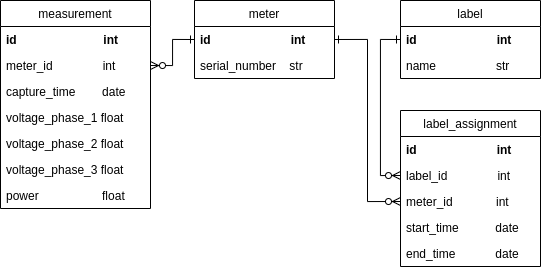
\includegraphics[width=1.0\textwidth]{gfx/smic-db}
    \caption{
        ER Diagramm der Datenbank
    }
    \label{fig:smic-db}
\end{figure}

Wie in Abbildung \ref{fig:smic-db} dargestellt, können in der Datenbank
die Verschiedenen Stromzähler mit ihrer Seriennumer abgespeichert werden.
Beispielsweise wird pro Haushalt ein Stromzähler mit einer bestimmten
Seriennummer abgespeichert, sobald dieser zum ersten mal Daten sendet.
Ein solcher Stromzähler sendet danach einzelne Messdaten zu bestimmten
Zeitpunkten. Die Messdaten beinhalten neben der Messzeit die drei Phasen
und wie viel Leistung gebraucht wurde.

Damit danach abgespeichert werden kann zu welcher Zeit beispielsweise ein
Toaster gelaufen ist, werden Labels erstellt. Ein solches Label hat eine
Bezeichnung und kann verschiedene Annotationen beinhalten.
Eine Annotation ist immer von einem bestimmten Stromzähler und kann implizit mehrere
Messdaten beinhalten. Dies wird über eine Start- und Endzeit abgespeichert.
Durch diese Struktur können danach einfach Auswertungen der Labels über mehrere
Stromzähler und Messpunkte gemacht werden.

\subsection{Architekturentscheidung}
\label{architekturentscheidung}

In dieser Arbeit wird keine Microservice Architektur im klassischen Sinne verwendet. (Siehe Kapitel \ref{konzepte:microservices})
Die einzelnen Komponenten werden zwar in separaten Container deployt (Abbildung: \ref{fig:smic-arch})
besitzen jedoch keine eigene Datenbank.
Das hat den Vorteil, dass weniger Overhead implementiert werden muss (mittels Message Queue)
und das Datenbankschema kann zentral in der Datastore Library einmal definiert
und dann in den verschiedenen Komponenten wiederverwendet werden.


\begin{figure}[h]
    \centering
    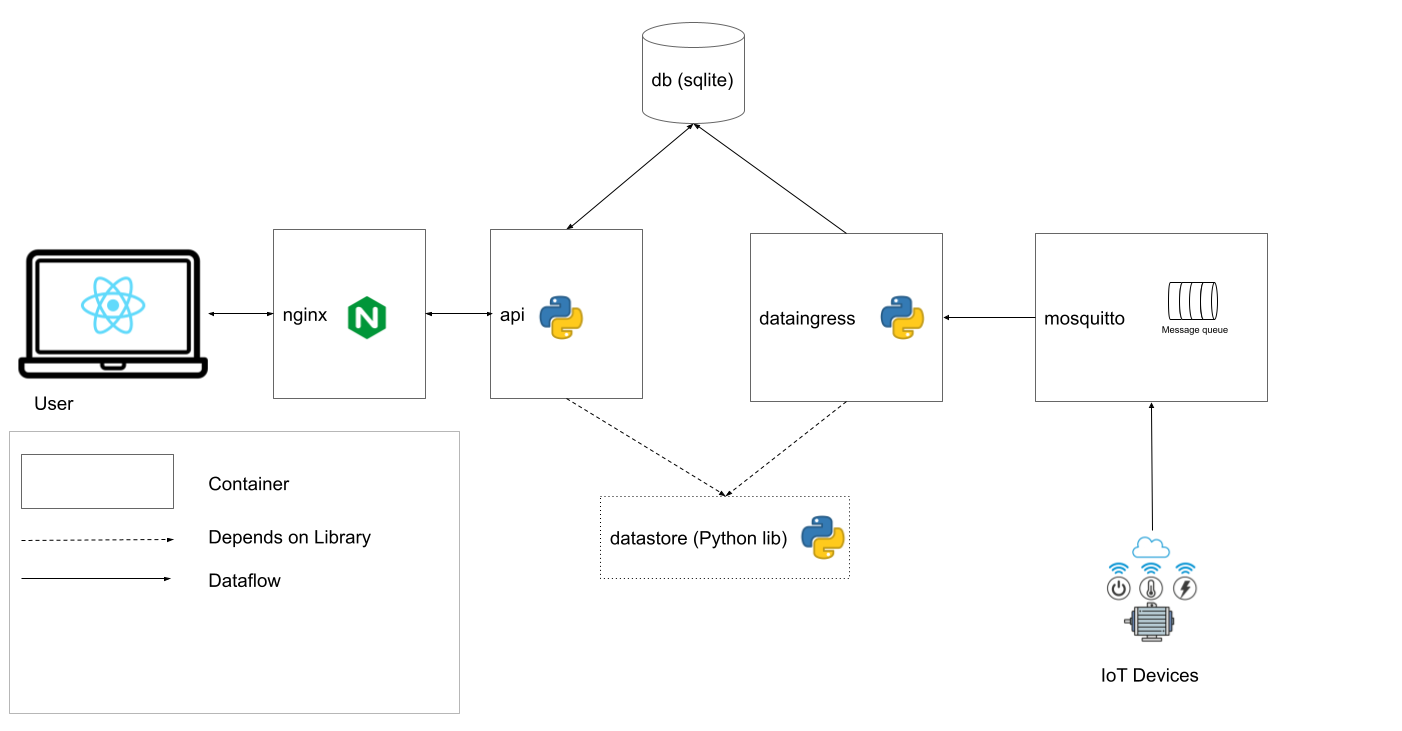
\includegraphics[width=1.0\textwidth]{gfx/smic-arch}
    \caption{
        Schematische Darstellung der in diesem Projekt verwendeten Architektur
    }
    \label{fig:smic-arch}
\end{figure}

Die Abbildung \ref{fig:smic-arch} zeigt die in diesem Projekt verwendete
Architektur auf. Hier noch einige Informationen zu den einzelnen Komponenten:


\begin{itemize}
    \item \texttt{nginx}:
        Alle Anfragen des Endbenutzers werden über einen Nginx Server
        entgegengenommen. Dieser liefert dann dem Benutzer die React WebApp
        oder leitet Anfragen an die \ac{API} weiter.

    \item \texttt{api}:
        Die \ac{API} verarbeitet Datenanfragen der React WebApp. Sie gibt
        beispielsweise die Stromzählerdaten eines Tages zurück.

    \item \texttt{datastore}:
        Der datastore ist eine Python library, die das Datenbankschema mittels \ac{ORM} festlegt.
        Sowohl die \ac{API} als auch der dataingress greifen auf die Datenbank zu
        und verwenden somit die datastore library.

    \item \texttt{dataingress}:
        Der dataingress arbeitet die von den \ac{IoT} Geräten gesendeten
        Stromzählerdaten ab und speichert diese in die Datenbank.

    \item \texttt{mosquitto}:
        Mosquitto ist der in dieser Arbeit verwendete \ac{MQTT} Broker.
\end{itemize}

Ein weiterer grund für die Entscheidung einer geteilten Datenbank ist,
dass der \texttt{dataingress} keine Daten liest, sondern diese nur von
der \ac{MQTT} Queue abarbeitet und in die Datenbank schreibt.

Auf die einzelnen Komponenten wird später in der Realisierungsphase noch genauer
eingegangen.

\subsection{Continous Integration, Contionous Delivery}

Um das Projekt automatisch Testen zu können und eine Reproduzierbare Umgebung zu bauen,
wurde bereits zu Beginn eine \ac{CI/CD} Pipeline mit GitHub Actions\footnote{https://github.com/features/actions}
aufgebaut.
Die Entwickler sollen sich nicht nur um die Entwicklung, sondern auch das automatische Bauen und Deployen der
Software kümmern. Dieser "DevOps" Gedanke hat den Vorteil, dass
theoretisch jedes kleine Feature und jeder Bugfix direkt automatisiert getestet
wird und danach (wenn die Tests erfolgreich waren) auf das Produktivsystem
Deployt werden kann. \cite{what_is_devops}
zudem ist für jeden Entwickler das Bauen und Ausführen des Projektes gleich und
reproduzierbar. Dies erspart das Suchen von unnötigen Fehlern die auf unterschiedlich
konfigurierten Entwicklungsmaschinen auftreten können.

\begin{figure}[h]
    \centering
    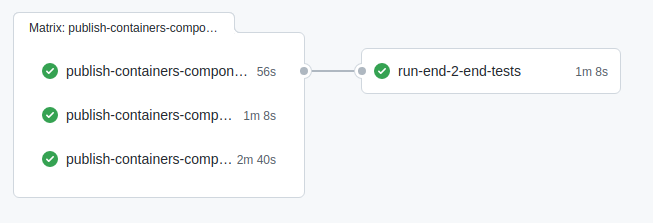
\includegraphics[width=1.0\textwidth]{gfx/ci-env}
    \caption{
        Visualisierung der GitHub Actions Pipeline mit zwei aufeinanderfolgenden Stages.
        Zuerst werden die einzelnen Komponenten (Siehe \ref{fig:smic-arch}) gebaut und
        anschliessend getestet.
    }
    \label{fig:ci-env}
\end{figure}

Dank dieser \ac{CI/CD} Umgebung und der Verwendung von Podman, kann die gesamte Applikation
(Wie im Kapitel \ref{architekturentscheidung} beschrieben) mit einem
Befehl gebaut und gestartet werden.


\section{Demo nach der ersten Phase}
Screenshot der ersten version
Rückmeldungen:
- grundsätzlich zufrieden
- Mobile nicht weiter zentral, Fokus auf Dashboard, Desktop

Neue Anforderungen:
Range/Zähler auswählen sowie typ der Daten
echte Daten automatisiert einspielen
THD und Power zusätzlich zu Spannung

\section{Demon nach der zweiten Phase}
- Labeling:
Labels graphisch darstellen
Labels mittels UI hinzufügen
